\documentclass[midd]{thesis}

\usepackage{graphicx}
\usepackage{times}

\bibliographystyle{plain}

\title {Computational Aesthetic Evaluation using Convolutional Neural Networks: Filtering Generative Art by Modeling User Tastes}

\author {Teddy Knox}
\adviser {Professor Christopher Andrews}

\begin{document}

\maketitle

\begin{abstract}
Recent advances in machine learning techniques have resulted in increasingly effective algorithms for discovering creative solutions to quantifiable optimization problems. In general, problems unaffected by advances in machine learning are not those involving creativity, but those whose optimization functions are difficult to quantify. To teach a computer to produce aesthetically pleasing artwork, one must first have in hand a model for aesthetic evaluation to guide the artwork generation. We performed several experiments with Convolutional Neural Networks to produce a hybrid Computational Aesthetic Evaluation model, and generate abstract art appealing to the user's tastes.
\end{abstract}

\begin{acknowledgements}
I dedicate this paper to science.
\end{acknowledgements}

\contentspage
\tablelistpage
\figurelistpage

\normalspacing \setcounter{page}{1} \pagenumbering{arabic}

\chapter{Introduction}
\label{sec:intro}

The accuracy of state of the art machine learning techniques have exceeded the accuracy of humans in certain limited tasks, and has . Using a state-of-the-art convolutional neural network \"out of the box\", we tested whether the modeling the statistically-defined visual aesthetic tastes of an individual. Our first trained model achieved 74\% accuracy in distinguishing aesthetically pleasing and displeasing abstract generative art, suggesting that deep learning techniques may be well-suited to the task of modeling the statistical distribution of arbitrary user tastes. In other words, the supervised techniques capable of recognizing a dog in an image may also be effective at recognizing a well-composed photograph. This presupposes Several difficult modeling tasks could soon be easier thanks to these advances. The task of computational aesthetic evaluation (CAE) is to judge the aesthetic value of a piece of artwork according to subjective criteria. The most groundbreaking advances on this task will likely stem from insights into the neural heuristics underpinning near-universal human preference for qualities such as consonance and composition, leading to new unsupervised learning techniques. Although these techniques will lay a foundation for more naturaly.

  Two ways to go:
  - Computational Aesthetic Evaluation
  - Recommendation systems


% Convolutional neural networks and the nature of training sets and computational aesthetic evaluation



% Old


Generative art is art produced using a well-defined procedures. The procedures need not be carried out by a computer. Early examples of generative art can be found in ancient pottery and religious decorations, often involving the tesselation of geometric shapes and colors. These early examples are impressive for their cerebral nature and the unusual human precision, but their scale and complexity were severely limited by the available human resources for  calculation and manufacture. With the invention of modern computers, the limiting factor on the increasing prevalance and complexity of generative art has become the artist, specifically their expertise in creative decision making and aesthetic evaluation. Despite their enormous computational power, the primary use of modern computers in generative art falls into the category of rendering procedures into their realized form, rather than participating in the search for aesthetic beauty. Advances in machine learning for pattern recognition have proved useful in many different types of well-defined tasks. In this study we apply modern image classification techniques using convolutional neural networks to the problem of computational aesthetic evaluation, observing whether they are capable of learning the tastes evident in a dataset of randomly generated triangle art, labeled with aesthetic quality ratings.

% - Not as much work in computer imagined art -- art which presents a few layers of abstraction so that each result is
% unique and valuable on its own
% - The goal, of course, when it comes to art is to produce beauty. But this in itself is not a simple concept.
%   The branch of philosophy called Aesthetics can lend us some insight into where to look for answers.
% - sensory tastes vary from person to person, although beauty is different as it is generally claimed as a universal
%   property of a thing.
% - Emanuel Kant argued that judgements of beauty are sensory, emotional and intellectual all at once,
%   as opposed to judgements of enjoyment which are purely sensory.
% - Contemporary views on beauty refuse such a thing as universal beauty, attributing such aesthetic certainties to the
%   power of culture to shape opinions similarly.
% - At the same time, it's fairly likely that humans have an innate disposition for certain aesthetics
%   - think musical consonance and disonance
%   - or facial or physical beauty for sexual reproduction (along with facial expressions)
%   - Some have theorized that aesthetic pleasure has to do with the resolution of apparent complexity into compressed
%     representations.
%     - If so, might it be possible to train a classifier to recognize these complex compositions
%       with compact representations.

% - We experiment with state-of the art Convolutional Neural Networks to predict the subjective aesthetic beauty.

\chapter{Related Work}

The focus of this study of computation aesthetic evaluation is composed of two parts: generative art and machine learning.

\section{Related Work in Generative Art}

Philip Galanter has done the most to rigorously define the problem of computational aesthetic evaluation. In his paper, Computational Aesthetic Evaluation: Steps Towards Machine Creativity, he lays out current difficulties with programing creativity into a computer ~\cite{galanter-3}.

Several others have applied genetic algorithms to optimize heuristics for aesthetic quality. For instance, a group
seeking to automatically generate layouts for page content used the heuristic of minimizing wasted space as a fitness
function on their population of layouts.

\section{Related Work in Image Classification}

\chapter{Theory}

\section{Generative Art}

Three factors went into the selection of the type of artwork to be used in this experiment. First, a body of art with a significant variance in subjective quality was desirable, since the experiment hinges on judging differences in quality. Next, a type of art with sufficiently simple characteristics was desirable to make the job of image classification as simple as possible without sacrificing the fundamental complexities of color scheme and composition. Last, in order to collect a large corpus of images quickly, an artform allowing for an efficient curation process was desirable. A corpus generative art lends itself nicely to these three constraints, since the randomness inherent tends to result in a variance in quality, the sophisitcation of abstract art is relatively low, and an endless pool of images can be sourced instantaneously.

I designed an extremely simple generative art method for producing our corpus of data. To produce an image, the program randomly places a random number of randomly-colored triangles on a randomly-colored background. I used a uniform random distribution in every case. I bounded the possible number of triangles, and limited the lightness of colors to a range, to boost the ratio of good results to bad results.

\section{Compuational Aesthetic Evaluation - Convolutional Neural Network}

We will use various CNN models that come with Caffe \"out of the box\" to test their efficacy, rather than attempt to customize a model to this task. The first model we will test is called GoogLeNet, which won the ImageNet Large Scale Visual Recognition Challenge in 2014.

\chapter{Implementation}

\section{Generative Art}

I designed a web interface for recording a binary rating to 4000 generated images, each three times, to form a composite score for each image. At each training interval, the trainer is shown an image on the screen, and asked to rate its quality as \"good\" or \"bad\". Sometimes the trainer is shown an image they have rated before, in order to corroborate the quality of the image.

The business logic of this training interface is written in python, because Caffe supports python bindings to its functionality. The images were drawn using the \"pillow\" python package. I opted not to use processing because I was unaware of any processing port to python.

% - Once we have a functioning model, we plan use it in the generation of new images to filter out bad random results.

\section{Compuational Aesthetic Evaluation - Convolutional Neural Network}

I chose to use the Caffe framework for image recognition for its documentation and widespread adoption in the machine learning community.

We will train GoogLeNet on a random subset of the images, and test it on the rest.

\chapter{Results}

I put together a training corpus of 4000 images, each with 3 binary ratings.

I plan to use standard metrics for measuring the effectiveness of our classifier.

I plan to use our model to filter ugly results from our triangle art generator and showcase the quality of the CAE model on free range images.

If time allows, I plan to feed different classes of artwork into the CAE model to test its efficacy at applying aesthetic preferences learned with the abstract shapes to forms of higher complexity.

\chapter{Conclusion}

Given the difficulty of defining art itself, it is no surprise that the criticism and reception of art itself is as nebulous. Yet despite the unclear underpinnings of aesthetic tastes, it is clear that aesthetic judgements are an integral part of everyday life. Short of machine intelligence, computerized judgements of aesthetics will likely never supercede our own, but in combination with our own, there is the potential for computers to make artists out of us all, or at least reduce the cost of aesthetically pleasing design.

The outcome of this experiment may not be clear and but the field of computational aesthetic evaluation will only gain in relevance as we strive to make our world more beautiful.

% - Is there a unifying aspect behind the beauty of various types of things?
% - Could we teach a computer to find a beautiful solution to a problem by studying how to generate beautiful artwork?
% - There have been much academic discussion of questions of where to begin with the problem of Computation Aesthetic Evaluation.
% - the general consesnus is: baby steps.
% - A deeply interconnected problem
%   - why?

Qualitative results here

% \chapter{Bibliography}
\bibliographystyle{plain}
\bibliography{thesis}
\cite{takagi, galanter-1, galanter-2, galanter-3}

% This thesis has many chapters.  For more on Alice see
% Chapter~\ref{sec:alice}, and in particular Section~\ref{sec:reproach}.
%
% \section{SECTION 1}
% The text for Section 1 goes here.
%
% \section{SECTION 2}
% Section 2 text.
%
% \subsection{Subsection heading goes here}
% Subsection 1 text
%
% \subsubsection{Subsubsection 1 heading goes here}
% Subsubsection 1 text
%
% \subsubsection{Subsubsection 2 heading goes here}
% Subsubsection 2 text
%
% \section{SECTION 3}
% Section 3 text. The dielectric constant at the air-metal interface
% determines the resonance shift as absorption or capture occurs.
%
% \begin{equation}
% \label{eqn:sampleEqn}
% k_1=\frac{\omega }{c({1/\varepsilon_m + 1/\varepsilon_i})^{1/2}}=k_2=\frac{\omega
% sin(\theta)\varepsilon_{air}^{1/2}}{c}
% \end{equation}
%
% \noindent
% where $\omega$ is the frequency of the plasmon, $c$ is the speed of
% light, $\varepsilon_m$ is the dielectric constant of the metal,
% $\varepsilon_i$ is the dielectric constant of neighboring insulator,
% and $\varepsilon_{air}$ is the dielectric constant of air.
% Equation~\ref{eqn:sampleEqn} makes this perfectly clear.
% See also Figure~\ref{fig:myfig} for an illustration.
%
%
% \begin{figure}
% \centering
% 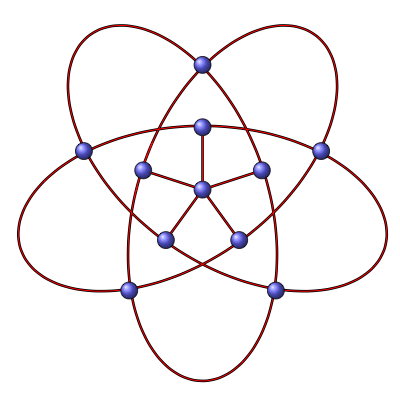
\includegraphics[width=0.75\textwidth]{graph.png}
% \caption{My figure.}
% \label{fig:myfig}
% \end{figure}
%
% \chapter{Alice in Wonderland}
% \label{sec:alice}
%
% \section{The Black Kitten}
%   One thing was certain, that the WHITE kitten had had nothing to
% do with it:---it was the black kitten's fault entirely~\cite{aiw}.  For the
% white kitten had been having its face washed by the old cat for
% the last quarter of an hour (and bearing it pretty well,
% considering); so you see that it COULDN'T have had any hand in
% the mischief.
%
%   The way Dinah washed her children's faces was this:  first she
% held the poor thing down by its ear with one paw, and then with
% the other paw she rubbed its face all over, the wrong way,
% beginning at the nose:  and just now, as I said, she was hard at
% work on the white kitten, which was lying quite still and trying
% to purr---no doubt feeling that it was all meant for its good.
%
%   But the black kitten had been finished with earlier in the
% afternoon, and so, while Alice was sitting curled up in a corner
% of the great arm-chair, half talking to herself and half asleep,
% the kitten had been having a grand game of romps with the ball of
% worsted Alice had been trying to wind up, and had been rolling it
% up and down till it had all come undone again; and there it was,
% spread over the hearth-rug, all knots and tangles, with the
% kitten running after its own tail in the middle.
%
% \section{The Reproach}
% \label{sec:reproach}
%
% (As promised in Chapter~\ref{sec:intro}, here it gets interesting.)
%
%   `Oh, you wicked little thing!' cried Alice, catching up the
% kitten, and giving it a little kiss to make it understand that it
% was in disgrace.  `Really, Dinah ought to have taught you better
% manners!  You OUGHT, Dinah, you know you ought!' she added,
% looking reproachfully at the old cat, and speaking in as cross a
% voice as she could manage---and then she scrambled back into the
% arm-chair, taking the kitten and the worsted with her, and began
% winding up the ball again.  But she didn't get on very fast, as
% she was talking all the time, sometimes to the kitten, and
% sometimes to herself.  Kitty sat very demurely on her knee,
% pretending to watch the progress of the winding, and now and then
% putting out one paw and gently touching the ball, as if it would
% be glad to help, if it might.
%
%   `Do you know what to-morrow is, Kitty?' Alice began.  `You'd
% have guessed if you'd been up in the window with me---only Dinah
% was making you tidy, so you couldn't.  I was watching the boys
% getting in stick for the bonfire---and it wants plenty of
% sticks, Kitty!  Only it got so cold, and it snowed so, they had
% to leave off.  Never mind, Kitty, we'll go and see the bonfire
% to-morrow.'  Here Alice wound two or three turns of the worsted
% round the kitten's neck, just to see how it would look:  this led
% to a scramble, in which the ball rolled down upon the floor, and
% yards and yards of it got unwound again.
%
%   `Do you know, I was so angry, Kitty,' Alice went on as soon as
% they were comfortably settled again, `when I saw all the mischief
% you had been doing, I was very nearly opening the window, and
% putting you out into the snow!  And you'd have deserved it, you
% little mischievous darling!  What have you got to say for
% yourself?  Now don't interrupt me!' she went on, holding up one
% finger.  `I'm going to tell you all your faults.  Number one:
% you squeaked twice while Dinah was washing your face this
% morning.  Now you can't deny it, Kitty:  I heard you!  What that
% you say?' (pretending that the kitten was speaking.)  `Her paw
% went into your eye?  Well, that's YOUR fault, for keeping your
% eyes open---if you'd shut them tight up, it wouldn't have
% happened.  Now don't make any more excuses, but listen!  Number
% two:  you pulled Snowdrop away by the tail just as I had put down
% the saucer of milk before her!  What, you were thirsty, were you?
%
% \chapter{Chapter 3}
%
% \chapter{Chapter 4}
%
% \appendix
% \chapter{Chapter 1 of appendix}
% Appendix chapter 1 text goes here

\end{document}
